% begin module limit-laws-ex4
\begin{frame}
\begin{example}[Example 4, p. 107]
Find $\lim_{x\to 1} g(x)$, where
\[
g(x) = \left\{ \begin{array}{lcl}
x + 1 & \text{ if } & x\neq 1 \\
\pi & \text{ if } & x = 1 
\end{array}\right.
\]
\uncover<2->{$g$ agrees with the function $f(x) = x + 1$ at every point except for $x = 1$.}
\uncover<3->{
\abovedisplayskip=0pt
\belowdisplayskip=0pt
\[
\lim_{x\to 1} g(x) = \lim_{x\to 1}(x + 1)= \uncover<4->{2.}
\]
}

\begin{center}
\begin{tabular}{cc}
\ \uncover<2->{%
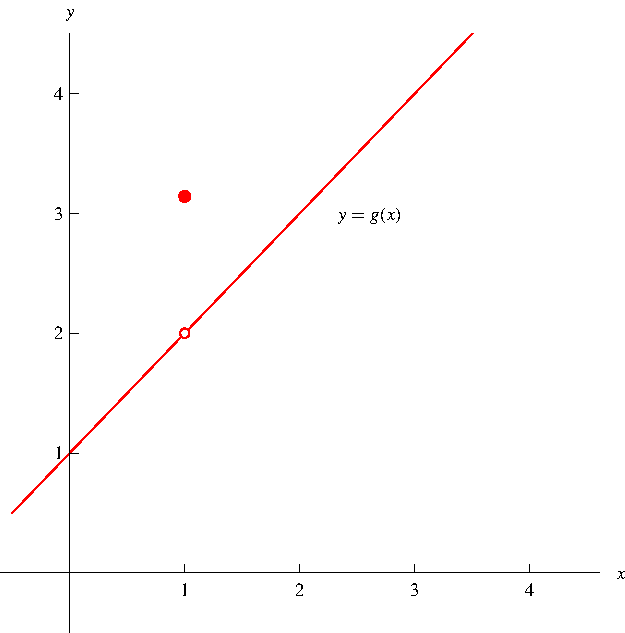
\includegraphics[height=3.5cm]{limits/pictures/02-03-ex4b.pdf}%
}%
&%
\ \uncover<2->{%
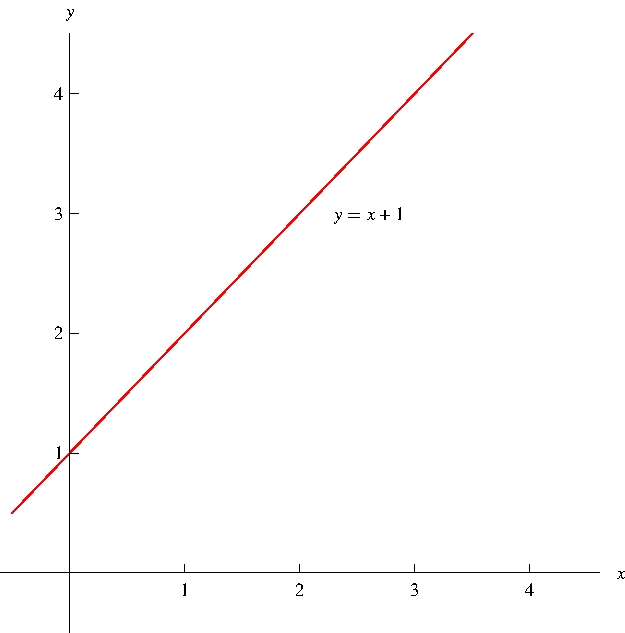
\includegraphics[height=3.5cm]{limits/pictures/02-03-ex4a.pdf}%
}%
\end{tabular}
\end{center}
\end{example}
\end{frame}
% end module limit-laws-ex4
